% This is samplepaper.tex, a sample chapter demonstrating the
% LNCS macro package for Springer Computer Science proceedings;
% Version 2.20 of 2017/10/04
%
\documentclass[runningheads]{llncs}
%
\usepackage{xcolor}
\usepackage{graphicx}
\usepackage{url}
\usepackage{makecell}
%\renewcommand\theadalign{bc}
\renewcommand\theadfont{\bfseries}
\renewcommand\theadgape{\Gape[4pt]}
\renewcommand\cellgape{\Gape[4pt]}

\graphicspath{ {./figures/} }

\usepackage{array, boldline, makecell, booktabs}
% Used for displaying a sample figure. If possible, figure files should
% be included in EPS format.
%
% If you use the hyperref package, please uncomment the following line
% to display URLs in blue roman font according to Springer's eBook style:
% \renewcommand\UrlFont{\color{blue}\rmfamily}

\begin{document}
%
\title{Classification of noisy free-text prostate cancer pathology reports using natural language processing\thanks{Supported by University of Applied Sciences Western Switzerland (HES-SO), Sierre, Switzerland.}}
\titlerunning{Classification of noisy free-text prostate cancer pathology reports using NLP}
% If the paper title is too long for the running head, you can set
% an abbreviated paper title here
% Henning: maybe we can mark the tentative author list here, so there is no discussion on this afterwards.
\author{Anjani Dhrangadhariya\inst{1}\orcidID{0000-0003-1691-1338} \and
Sebastian Otálora\inst{1}\orcidID{0000-0003-2125-8476} \and
Manfredo Atzori\inst{1}\orcidID{0000-0001-5397-2063} \and Henning M\"uller\inst{2}\orcidID{0000-0001-6800-9878}}
%
\authorrunning{A. Dhrangadhariya et al.}
% First names are abbreviated in the running head.
% If there are more than two authors, 'et al.' is used.
%
\institute{University of Applied Sciences Western Switzerland (HES-SO), Sierre, Switzerland \email{anjani.dhrangadhariya@hevs.ch} \and
University of Geneva (UNIGE), Geneva, Switzerland}
%
\maketitle              % typeset the header of the contribution
%
\begin{abstract}
Free-text reporting has been the main approach in clinical pathology practice for decades. 
Pathology reports are an essential information source to guide the treatment of cancer patients and for cancer registries, which process high volumes of free-text reports annually. Information coding and extraction are usually performed manually and it is an expensive and time-consuming process, since reports vary widely between institutions, usually contain noise and do not have a standard structure.
This paper presents strategies based on natural language processing (NLP) models to classify noisy free-text pathology reports of high and low-grade prostate cancer from the open-source repository TCGA (The Cancer Genome Atlas). 
We used paragraph vectors to encode the reports and compared them with \textit{n}-grams and TF-IDF representations. The best representation based on distributed bag of words of paragraph vectors obtained an $f_{1}$-score of 0.858 and an AUC of 0.854 using a logistic regression classifier. We investigate the classifier's more relevant words in each case using the LIME interpretability tool, confirming the classifiers' usefulness to select relevant diagnostic words. Our results show the feasibility of using paragraph embeddings to represent and classify pathology reports. 
\keywords{Pathology Reports  \and Natural Language Processing \and Paragraph Embeddings}
\end{abstract}
%
\section{Introduction}
%
Pathologists examine tissue via a microscope or in a digital image looking for specific cell and gland morphologies that resemble cancer or healthy tissue. After careful examination, they summarize their findings in a free-text report, as shown in Figure~\ref{fig:reports}. Pathology reports include a diagnosis or a score in a grading/staging system, despite being an inherently complex and uncertain process~\cite{PPA2009}. The outcomes are often discussed in tumor boards or given to oncologists and referring clinicians to decide on the best treatment options for the patient.

While free-text reporting has been the main approach in clinical practice for decades (sometimes helped by speech recognition), structured reporting is gaining importance in clinical practice, as it allows to improve quality parameters in diagnostic practice, including timeliness, accuracy, completeness, conformance with current agreed standards, consistency and clarity in communication.
In addition, structured approaches can be fundamental (e.g. for cancer registries) for population-level quality monitoring, benchmarking, interventions and benefit analyses in public health management~\cite{ellis2016does}.

Automatic analysis and classification of reports can allow to enhance the practice of pathologists.
First, it is a possible way to create structured reports from free text ones, in order to standardize previously diagnosed cases for monitoring, benchmarking and benefit analyses in public health management.
Second, it can allow to retrieve similar cases in proprietary databases ~\cite{schaer2019deep}, enabling pathologists to navigate repositories of images for clinical decision support and teaching. In such situations, the comparison with visually similar cases is fundamental to reduce the risk of misinterpretations in the diagnosis and provide high quality teaching guidelines.
Finally, it can allow faster preparation of multi-center and population-level studies, which require a single agreed international and evidence-based standard to ensure interoperability and comparability~\cite{ellis2016does}.

Manually extracting information from free-text pathology reports is an expensive and time-consuming process since they vary widely between institutions, usually contain noise and do not have a standard structure.
Still, manual extraction is the most common practice when structured reports are not available, since free-text reports are in most cases extremely noisy and the design and creation of tools that automatically extract information from pathology reports is not straightforward ~\cite{OAK2020,CHG2019,del2017convolutional}. 
With the advent of digital pathology and structured reporting, there is an increasing interest in automatic analysis of pathology reports~\cite{BNF2019,YBS2017,QYF2017,GYQ2018,XCS2018}.
%
\begin{figure}
\label{fig:reports}
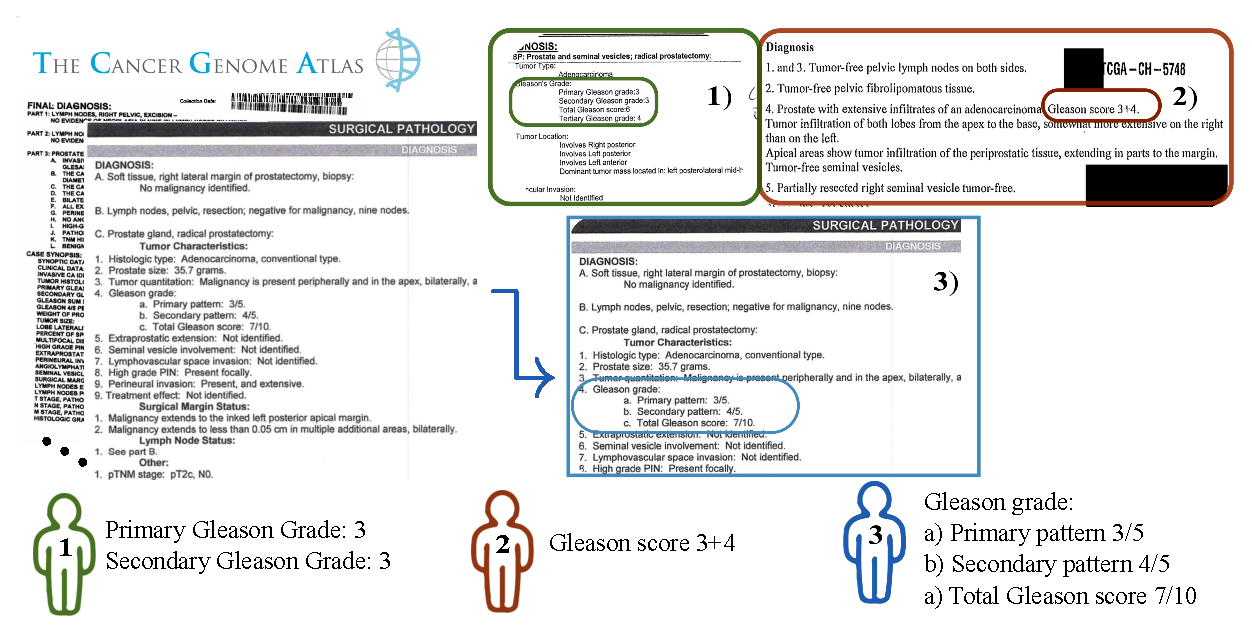
\includegraphics[width=\textwidth]{examples_reports.eps}
\caption{Snippets of three pathology reports from the TCGA-PRAD repository. The variation in the diagnosis text makes it difficult to manually develop specified rules to extract these important parts of the report automatically.} 
\end{figure}
%

Natural Language Processing (NLP) tools are used extensively to analyze clinical health records automatically~\cite{YBS2017,OMS2020,GYQ2018}.  While there has been an increase in the use of recurrent neural networks~\cite{GYQ2018} and word2vec embeddings~\cite{JOA2017a} to represent the content of reports, the use of deep learning techniques has not yet fully penetrated clinical NLP~\cite{WRD2020}. Particularly, with the recently proposed distributed representations of words and documents~\cite{le2014distributed}, and transformer networks that have outperformed traditional NLP approaches in many NLP tasks and benchmarks~\cite{VSP2017}, the evidence on the applicability to clinical and pathology text remains under-explored.

\section{Related Work}
%
There are machine learning and NLP approaches in the literature that classify and extract clinical information from pathology reports~\cite{GYQ2018} automatically. The tasks' performance varies widely and depends mainly on the database's size of the database and how structured the reports are.
In the work of Yala et al.~\cite{YBS2017}, each of the sentences in a large dataset of more than 90,000 breast cancer pathology reports is represented with an n-gram. Each report is classified independently into 20 categories, with an average accuracy of 97\%.
In the work of Qiu et al.~\cite{QYF2017}, the authors use a CNN to automatically extract ICD-O-3 topographic codes from a corpus of breast and lung cancer pathology reports, obtaining a micro-F score of 0.811 and outperforming conventional NLP strategies. 
Gao et al.~\cite{GYQ2018} used hierarchical attention networks to model free-text pathology reports and extract from them information, including primary tumor sites and histological grades, obtaining macro F-scores of 0.852 and 0.708 respectively in a set of 942 pathology reports.
%In contrast, in radiology, several approaches deal with short, well-structured reports~\cite{SWM2020}.
%~\cite{ZZZ2019}
In the work of Alawad et al.~\cite{AGQ2020}, the authors used a multitask CNN for classifying histological grade, type, laterality, and primary cancer site in a dataset of 95231 pathology reports, achieving a macro-F measure of 0.766 in the grading task. 
Similar studies usually lack an in-depth analysis of the classifier's more relevant words, besides reporting the model's quantitative performance. 
This paper investigates the use of paragraph vectors to represent and classify high and low-grade prostate pathology reports.
We encode the reports using distributed representations of sentences and compare it to standard NLP techniques. Our results show that our approach is better than conventional and TF-IDF by 0.23 in AUC, reaching an F-score of 0.858 and an AUC of 0.854. We also analyze the more relevant words qualitatively for classifying the reports in each class, finding them similar to the words that pathologists use the diagnosis of Gleason grading. %
%
\section{Methods}
\label{sec:methods}
%
This section describes the pathology report corpus used, the pre-processing steps and the classification approach.
Figure~\ref{fig:approach} gives an overview of our approach used to automatically classify pathology reports into high-grade vs. low-grade prostate cancer.
%
\begin{figure}[h!]
    \centering
    \includegraphics[scale=0.40]{figures/preprocessing.png}
    \caption{Our approach} %Hdenning: the figure requires a caption that describes the figure and is meaningful. Two words are not sufficient
    \label{fig:approach}
\end{figure}
%
\subsection{Corpus}
\label{subsec:dataset}
%
The approach described in this paper uses publicly available prostate adenocarcinoma clinical pathology reports from The Cancer Genome Atlas (TCGA) PanCancer dataset~\footnote{\url{lhttps://portal.gdc.cancer.gov/projects/TCGA-PRAD}}.
The clinical report corpus originally consisted of 494~\footnote{\url{http://www.cbioportal.org/study/clinicalData?id=prad_tcga_pan_can_atlas_2018}} reports out of which 404 non-empty reports were selected for further analysis.
These reports were varying in length (see Figure~\ref{fig:datasetchar}), unstructured free-text (see Figure~\ref{fig:reports}) scanned copies of the original documents available as Portable Document Format (PDF).
An unstructured report in contrast to a structured report is not divided into self-explanatory sections.
The corpus documents were manually labelled with two class labels: high-grade (Gleason Score >7) and low-grade (Gleason Score < 6,7) using the diagnosis information from them. This separation has clinically relevant patient stratification~\cite{NBG2001}.
After manual classification, 171 reports were identified as high-grade prostate cancer and 233 reports were identified as low-grade prostate cancer creating a slight class imbalance (refer Figure~\ref{fig:datasetchar}).
%
\subsection{Corpus preprocessing}
\label{subsec:preproc}
%
Any text corpus requires thorough preprocessing before it can be used for any downstream NLP task. 
Text preprocessing primarily includes 1) conversion of immutable text documents to machine readable, 2) filtering of useless and noisy parts from the data, and 3) removal of uninformative filler words.
The following preprocessing steps were performed before the feature extraction.
%
\paragraph{1. PDF to text: } The PDF documents were converted into editable and searchable text files using GOCR, an open-source optical character reader (OCR) data suite~\footnote{\url{http://jocr.sourceforge.net/}}.
%
\paragraph{2. Fixed-pattern noise removal: } Next, the most apparent noise elements following a known pattern, like a trail of hyphens (-), pipes ($\vert$), asterisks (*), patient identifiers (for e.g., Patient ID: QUID : 70DD94DF - 1301 . 40FC-A52B - 43E2229563E3), sample identifiers (for e.g., TCGA- ZG-A9NI - 91A-PR), and HEX NULL characters (e.g. $<$0x0C$>$, $<$0x0F$>$) were automatically removed.
Fully automatic filtering can miss some noise.
Denoising these documents was an important preprocessing step.
%
\paragraph{3. Stop-word removal: } The most frequent, noisy tokens were automatically removed using a set of predefined English language stop-words provided by NLTK (Natural Language ToolKit)~\footnote{\url{https://www.nltk.org/api/nltk.tokenize.html}} along with the corpus-specific stop-words and punctuation, listed in Table~\ref{tab:stopwords}.
%
\begin{table}[]
    \centering
        \caption{List of the additional corpus-specific stop-words removed from the pathology reports.}
        \begin{tabular}{ |p{2cm}|p{2cm}|p{2cm}||p{0.8cm}|p{0.8cm}|p{0.8cm}|p{0.8cm}|p{0.8cm}| } 
         \hline
         \multicolumn{3}{|c||}{Stop-words} & \multicolumn{5}{|c|}{Punctuation}  \\
         \hline
         report & reviewed & surgical & ; & \# & [] & ` & . \\
         \hline
         electronically & approved & signed & : & () & ? & / & \& \\ 
         \hline
         pathology & page & redacted & , & \_  & ! & \textbackslash & " \\ 
         \hline
        \end{tabular}
    \vspace{1mm}
    \label{tab:stopwords}
\end{table}
%
\subsection{Data Augmentation}
\label{subsec:aug}
%
Class imbalance often reduces the classifier performance, so in the present work it was addressed by oversampling through back-translation text augmentation technique.
Augmentation and oversampling using back-translation process involves augmenting the minority class by translating a document to a language other than the source language and then translating it back to the source language~\cite{WLV2020}.
Here the documents were translated from the source language English to German and back using the Google translate python package~\footnote{\url{https://pypi.org/project/googletrans/}}.
German was used as a target language for augmentation because it has a high lexical similarity with English (a similarity coefficient of 0.60) thereby adding variability to the oversampled text without altering its meaning~\cite{lexical}.
%Anjani: We use German because it shares the Saxon roots of English, adding variability, but not too much

The corpus was split into training and test sets. After splitting, the training set was oversampled to equally learn both the classes during training. Table~\ref{tbl:dataset} gives a summary of the corpus used in our experiments.
%
\begin{table}
\begin{center}
\caption{Number of reports per class after train-test split and oversampling.}\label{tbl:dataset}
\begin{tabular}{|c|c|c|c|}
\hline
Partition/Class &   Train & Test\\
\hline
High-Grade & 186 & 47\\
\hline
Low-Grade & 186 & 34\\
\hline
\end{tabular}
\end{center}
\end{table}
%
\subsection{Document Representation}
\label{subsec:doc_rep}
%
In natural language classification problems, it is important to represent the text documents in machine understandable form.
Text representation or vectorization methods convert text documents into fixed-length numeric vectors understood by NLP systems.
Two types of numeric representations were extracted from the documents, each one encoding different levels of information.
These text representation methods were: I) Count-based vectors, and II) Semantic vectors.
%
\paragraph{Count vectors: } 
%
Count vectors encode text as word counts or frequency.
Term Frequency - Inverse Document Frequency (TF-IDF) is weighted, sparse, word frequency encoding for numeric text representation.
TF-IDF is a multiplication between term frequency (TF) matrix and inverse document frequency (IDF) matrix.
Term frequency of a word $W$ is defined as the word count of $W$ for the document $D$ divided by the number of words $N$ in $D$.
IDF of a word $W$ is defined as logarithm of the total number of documents divided by the number of documents containing $W$.
tf-idf increases weight for the meaningful words in the corpus and reduces the weight for filler words like a, an, the, in, if, \textit{etc}~\cite{dhrangadhariya2020exploiting}.
%
\paragraph{Semantic vectors: }
%
Count vectors not only lose the word order and semantic information but also suffer high-dimensionality and sparsity. 
To take into account semantics of the text, document-level, semantic, dense paragraph vectors were extracted.
Paragraph vectors are generated in an unsupervised manner and learn a distributed representation for pieces of text along with distributed representation for the individual words.
These vectors learn to associate words with document identifiers rather than with the other words in the context.
This work used two kinds of paragraph vectors: 1) a distributed memory model of paragraph vectors (PV-DM) and
2) a distributed bag of words model of paragraph vectors (PV-DBOW)~\cite{le2014distributed}.
PV-DM and PV-DBOW vectors were generated for the training documents on fly during the experiments using the gensim functionality~\footnote{\url{https://radimrehurek.com/gensim/models/doc2vec.html}}.
%
\subsection{Document classification}
\label{subsec:trainingeval}
%
After feature extraction for each document, L2 normalization for each feature vector was computed.
All the labelled documents were used to train and evaluate multiple classifiers (Logistic Regression (LR), Support Vector Machines (SVMs) with linear kernel and K-nearest neighbour (KNN)) in order to separate the reports into high \textit{vs.} low-grade prostate cancer.
Grid search was used to explore and identify best performing parameters for these classifiers and feature vector combinations.
The model performance was evaluated on an independent held-out test set.
%
\subsection{Experimental setup}
\label{sec:experiments}
%
Twelve experiments were conducted each combining the above-mentioned feature vector-classifier combination.
Grid search was used to identify the best feature vector, hyperparameters and classifier combination in the training set using ROC AUC (Receiver Operating Curve; Area Under Curve) as a guiding metric.
The macro-F1 score, Precision, Recall and ROC AUC measures were used.
Random seed for the experiments was set to 42.
%
\paragraph{Hyperparameter space for count vectors: } 
%
The tf-idf vectors were extracted and an $n$-gram space with $n$ ranging from 1 to 10 was explored.
Too frequently or too infrequently appearing terms were controlled.
%
\paragraph{Hyperparameter space for semantic vectors: } 
%
For the semantic paragraph vectors, vector dimensions of 100, 300, and 500 with window sizes 2, 3 and 5.
The paragraph vectors were trained for epochs 20, 30 and 50 along with the above vector dimension and window size combination.
%
\section{Results}
\label{sec:results}
%
Table~\ref{tab:results} reports classification results for the best feature vector classifier combination.
Paragraph vectors capture better discriminatory information between the classes compared to the count vectors as seen from the ROC AUC scores.
PV-DBOW - logistic regression has the best ROC AUC score of 85.4\% compared to the other feature vector classifier combinations.
Compared to SVM classifier combined with paragraph vectors, LR offers gains in precision by 2.6\%, while the recall values for both the classifiers remain identical (79.4\%).
Paragraph vectors achieve this best ROC AUC score for the denoised, augmented and class-balanced training documents, but training with noisy documents leads to a massive drop in ROC AUC by 11.5\%.
Training these noisy documents without any oversampling leads to a further drop in ROC AUC by 2.6\%.
The confusion matrix for both the best performing feature vector - classifier combination is shown in Figure~\ref{fig:cm}. 
The hyperparamters for the best performing feature vectors are shown in Table~\ref{tab:hp}.
For the tf-idf vectors, KNN classifier offers overall better macro precision and recall compared to the other classifiers.
%
\begin{table}[]
    \centering
    \caption{The table shows the results for the best classifier-feature vector combination (see section~\ref{sec:experiments}).}
    \begin{tabular}{ p{3.5cm}m{1.5cm}m{1cm}m{1cm}m{1.5cm}m{1cm}m{1cm}m{1cm}  }
    \Xhline{1pt}
      & \multicolumn{3}{c}{class ``High-grade''} & \multicolumn{3}{c}{Macro average} & \\
    \Xhline{1pt}
     Feature-Classifier & Precision & Recall & F1 & Precision & Recall & F1 &  ROC AUC \\
    \Xhline{1pt}
     tf-idf-LR & 0.630 & 0.500 & 0.554 & 0.657 & 0.644 & 0.645 & 0.645 \\
     tf-idf-SVM & 0.655 & 0.559 & 0.603 & 0.683 & 0.683 & 0.675 & 0.673 \\
     tf-idf-KNN & 0.739 & 0.500 & 0.596 & 0.723  & 0.686 & 0.689 & 0.686 \\
     PV-DBOW-KNN & 0.826 & 0.559 & 0.667 & 0.784 & 0.737 & 0.743 & 0.737 \\
     PV-DBOW-SVM & 0.844 & \textbf{0.794} & 0.818 & 0.850 & 0.844 & 0.847 & 0.843 \\
     PV-DBOW-LR &  &  &  &  &  &  & \\
     - Denoised oversampled & \textbf{0.870} & \textbf{0.794} & \textbf{0.830} & \textbf{0.866} & \textbf{0.854} & \textbf{0.859} & \textbf{0.854} \\
     - noisy reports & 0.847 & 0.579 & 0.688 & 0.767 & 0.739 & 0.732 & 0.739 \\
     - no oversampling & 0.735 & 0.658 & 0.694 & 0.716 & 0.714 & 0.713 & 0.713 \\
    \Xhline{1pt}
    \end{tabular}
    \label{tab:results}
\end{table}
%
%
%
\begin{table}[]
    \centering
    \caption{The table shows the parameter settings used for the best feature vector-classifier combination (refer section~\ref{sec:experiments}).}
    \begin{tabular}{ p{2cm}p{1.5cm}p{7cm} }
    \Xhline{1pt}
     Features & Classifier & Vector parameters \\
    \Xhline{1pt}
     tf-idf & KNN & n-gram 10, max df 0.7, min df 0.0 \\
     PV-DBOW & LR &
         window size 5,
         vector dimension 300,
         epochs 20 \\
    \Xhline{1pt}
    \end{tabular}
    \label{tab:hp}
\end{table}
%
%
%
\begin{figure}
    \centering
    \includegraphics[scale=0.35]{figures/merge_confusionMatrix.jpg}
    \caption{Confusion matrix for best count vector classifier combination vs. best semantic vector classifier combination}
    \label{fig:cm}
\end{figure}
%
\section{Discussion \& Analysis}
\label{sec:disc}
%
\paragraph{The corpus characteristics:} The corpus with pathology reports consisted of highly variable length reports.
These are unstructured reports without any explicit demarcation or order for different sections like patient history, diagnosis, conclusion and summary.
Figure~\ref{fig:datasetchar} shows a histogram of the number of reports against report length measured in number of characters.
The smallest report had 485 characters while the longest one had 11440.
Additionally, except diagnosis section, not all reports were complete and comprehensive lacking one or the other above mentioned sections.
The reports originated from heterogeneous sources and were available in the PDF format.
Upon conversion from PDF to text format using open-source OCR software, further added to the noise to the already heterogeneous corpus.
All these issues made the preprocessing and classification process rather challenging.
\begin{figure}[h!]
  \centering
  \begin{minipage}[b]{0.4\textwidth}
    \includegraphics[width=\textwidth]{figures/varyingreportlengths.png}
    \caption{The graph shows report length for non-empty reports in terms of characters.}
  \end{minipage}
  \hfill
  \begin{minipage}[b]{0.4\textwidth}
    \includegraphics[width=\textwidth]{figures/high_low_imbalance.png}
    \caption{Histogram showing class imbalance in the corpus. ``0'' corresponds to class low-grade prostate cancer and ``1'' correspond to class high-grade prostate cancer.}
    \label{fig:datasetchar}
  \end{minipage}
\end{figure}
%
%
%
\paragraph{Interpretation: }
%
Paragraph vectors being based on shallow neural networks are considered as black-box representations.
In order to inspect if the best performing paragraph vector representations did capture relevant hints for classifying the documents into high \textit{vs.} low-grade prostate cancer, we used LIME (Local Interpretable Model-Agnostic Explanations).
LIME abstracts the behavior of a classifier around individual predicted instances in the form of interpretable natural language units i.e. the words.
LIME was used to extract six explanations for each class from the individual reports in the test set. 
Figures~\ref{fig:LIME0}, ~\ref{fig:LIME00},~\ref{fig:LIME1}, and~\ref{fig:LIME2} show LIME explanations for the high-grade and low-grade prostate cancer classes on the test instances.

Figure~\ref{fig:LIME0} shows a high-grade instance with LIME explanations for both the classes.
LIME picks up the numbers ``4'', ``5'', and ``9'' from the text which forms the part of gleason score phrase.
Total gleason grading score of ``9'' is one of the strongest clues to classify the diagnosed prostate cancer into high-grade.
\begin{figure}[h!]
    \centering
    \includegraphics[scale=0.3]{figures/highGrade_strong.png}
    \caption{LIME explanation for a high-grade report instance from the test set.}
    \label{fig:LIME0}
\end{figure}
%

In Figure~\ref{fig:LIME00}, we present a contradictory example where for a high-grade prostate cancer report, LIME confidently picks up rather irrelevant terms (right, left, prostatic, etc.) for the low-grade class instead.
%
\begin{figure}[h!]
    \centering
    \includegraphics[scale=0.3]{figures/irrelevant.png}
    \caption{LIME explanation for a high-grade report instance from the test set.}
    \label{fig:LIME00}
\end{figure}
%

Figure~\ref{fig:LIME1} shows low-grade instance with LIME explanations for the low-grade class.
One of the relevant explanation for classification into low-grade are the numbers ``3'', ``4'', and ``7''.
These numbers form part of the total gleason score term for low-grade prostate cancer.
The model, however, does not pick any word explanations from the class high-grade and also picks other irrelevant explanations like the term ``prosectomy'' and ``excision''.
%
\begin{figure}[h!]
    \centering
    \includegraphics[scale=0.3]{figures/strong_lowgrade.png}
    \caption{LIME explanation for a low-grade report instance from the corpus.}
    \label{fig:LIME1}
\end{figure}
%

Figure~\ref{fig:LIME2} shows a low-grade instance with several strong explanations.
For the class low-grade, several relevant clues are picked up; the tumor histologic grade term ``g3'' and the numbers ``3'' and ``4''. 
It can be noticed that these numbers form part of the Gleason grade phrases and are present in the reports as ``gleason grade 3+3'', ``gleason grade 3+4'', ``primary gleason grade 3'', ``secondary gleason grade 4'' depicting an overall low-grade Gleason score.
%
\begin{figure}[h!]
    \centering
    \includegraphics[scale=0.30]{figures/superStrongLowGrade.png}
    \caption{A strong LIME explanation for a low-grade report instance from the corpus.}
    \label{fig:LIME2}
\end{figure}
%

From each example LIME explanation demonstrated here, it has to be noted that the paragraph representation model picks several strong informative terms for each class but also picks up many irrelevant words with high confidence and misses out on rather strong diagnosis information terms.
LIME explanations warrant further inspection with respect to the hyper-parameters like the number of explanations generated, number of neighbouring samples used to generate explanations, random seed used, and distance metric~\cite{madhyastha2019model}.
%
\section{Conclusions \& future work}
\label{sec:conc}
We presented an approach for classification of noisy, heterogeneous pathology reports corpus into high-grade prostate cancer and low-grade prostate cancer using two levels of textual information. 
Semantic information proved to be more discriminatory between the classes compared to the count information.
%Conclusion: Best method, best output, problems
These pathology reports included unstructured complex information that is spread over long segments of text. 
Our results and interpretability analysis suggest not only the feasibility, but also reliability of using paragraph vectors to represent and classify prostate pathology reports into high- vs. low-grade prostate cancer.


%Future work
Each report consists of multiple tumor staging terms, clinical measurements, prostrate tissue anatomy information and their combination with negation terms.
We hypothesize that this problem of extracting information from pathology reports might be better suited as an entity recognition problem. Extracting semantically inclined entities could help fine-grained classification of these rather noisy, heterogeneous reports. 
The noisy and denoised prostrate cancer pathology report corpus, the source code to reproduce our experiments and the python notebook to explore interpretability analysis can be found on Github: \url{https://github.com/anjani-dhrangadhariya/pathology-report-classification.git}.  %Each term helps decide the final accurate staging for the detected tumor which goes beyond the binary high- vs. low-grade classification~\footnote{\url{https://cancerstaging.org/references-tools/quickreferences/Documents/ProstateSmall.pdf}}
%
% ---- Bibliography ----
%
% BibTeX users should specify bibliography style 'splncs04'.
% References will then be sorted and formatted in the correct style.
%
\section{Acknowledgements}
This project has received funding from the European Union's Horizon 2020 research and innovation program under grant agreement No 825292 ExaMode.  Sebastian Ot\'{a}lora thanks Minciencias through the call 756 for PhD studies.
\bibliographystyle{splncs04}
\bibliography{bibliography}
%longitudinal analysis
\end{document}
